\begin{frame}
    \frametitle{前情回顾}
    {\Bullet} 经典描述: 一个自由度为$n$的系统可以由成对的变量($q_1, q_2, \cdots, q_n, p_1, p_2, \cdots, p_n$)描述。$q_i$为广义坐标,$p_i$为广义速度。哈密顿有正则表示$H(q_1, q_2, \cdots, q_n, p_1, p_2, \cdots, p_n) $ 。每一组正则共轭变量($q_i, p_i$)符合哈密顿正则方程:
    \[ \frac{\mathrm{d} q_i }{\mathrm{d} t}  = \frac{\partial H }{\partial p_i}, \quad \frac{\mathrm{d} p_i }{\mathrm{d} t}  = - \frac{\partial H }{\partial q_i}\]
    {\Bullet} 正则量子化: 
    \begin{itemize}
        \item 写出经典哈密顿 H
        \item 哈密顿正则化
        \item 正则变量不对易, 算符化; 哈密顿算符化.
        \item 把哈密顿算符代入薛定谔方程求解.
    \end{itemize}     
\end{frame}

%%%%%%%%%%%%%%%%%%%%%%%%%%%%%%%%%%%%%%%%%%%%%%%%%%%%%%%%%%%%%
\begin{frame} [plain]
    \frametitle{}
    \Background[1] 
    \begin{center}
    {\huge 第4讲:光场量子化}
    \end{center}  
    \addtocounter{framenumber}{-1}   
\end{frame}
%%%%%%%%%%%%%%%%%%%%%%%%%%%%%%%%%%%%%%%%%%%%%%%%%%%%%%%%%%%% 


\section{1. 单模光场的量子化}

\begin{frame}
      \frametitle{电磁场的单模展开}
    考虑空腔中的一个线性极化的电磁波,如图 
    \begin{center}
     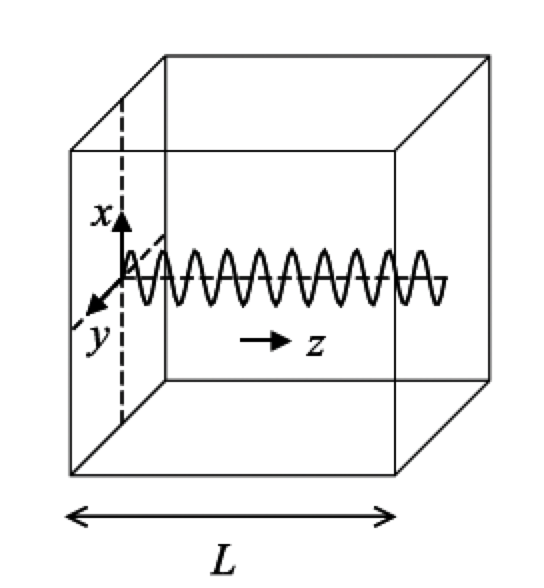
\includegraphics[width=0.20\textwidth]{figs/2022-04-27-12-37-33.png}
    \end{center}
    电磁场的能量密度: 
    \[ \omega = \frac{1}{2} (\epsilon_0 E^2 _x + \mu_0 H^2 _y) \]
    总能的经典哈密顿
    \[ H = \frac{1}{2} \int_V (\epsilon_0 E^2 _x + \mu_0 H^2 _y) dV \]      
\end{frame}

\begin{frame}
      \frametitle{}
    经典解为:
      \begin{enumerate}
        \IItem 电场叠加解:$\displaystyle E_{x}(z,t) = \sum\limits_{n=1}^{\infty } E_{0}  \sin \omega_n t \sin k_n z= \sum\limits_{n=1}^{\infty } a_n q_n (t) \sin (k_n z)$
        \IItem 磁场叠加解: $\displaystyle H_{y}(z,t) = \sum\limits_{n=1}^{\infty } H_{0}  \cos \omega_n t \cos k_n z = \sum\limits_{n=1}^{\infty } a_n \frac{\epsilon_0}{k_n}q_n ' (t) \cos (k_n z)$  
    \end{enumerate}	
    三维叠加解
    \[ \begin{aligned}
    \mathbf{E}( \mathbf{r},t) =& - \frac{1}{\sqrt{ \epsilon_0}} \sum_l ^\infty   q_l(t) \mathbf{E}_l( \mathbf{r}) \\
    \mathbf{H}( \mathbf{r},t) =&  \frac{1}{\sqrt{ \mu_0}} \sum_l ^\infty  \omega_l p_l(t) \mathbf{H}_l( \mathbf{r}) \\
    \end{aligned} 
    \] 
\end{frame}

\begin{frame}
      \frametitle{}
    代入电磁场的哈密顿量, 利用腔模正交性, 得:
    \[ \begin{aligned}
        H &= \frac{1}{2} \int_V (\mu_0 \mathbf{H}^2 + \epsilon_0 \mathbf{E}^2) dV \\ 
        &= \sum_l  \frac{1}{2}(p_l ^2 + \omega_l ^2 q_l ^2 ) \\ 
        &= \sum_l H_l  
     \end{aligned} 
    \] 
    电磁场哈密顿量是单模哈密顿量的线性叠加, 因此只要对单模进行量子化.
\end{frame}

\begin{frame}
      \frametitle{单模量子化}
      单模的哈密顿
      \[ H_l  =  \frac{1}{2}(p_l ^2 + \omega_l ^2 q_l ^2 ) \]
      写出密顿运动方程
    \[ \begin{aligned}
        \frac{\mathrm{d}p_l}{\mathrm{d}t} &= - \frac{\partial H_l}{\partial q_l} = - \omega ^2 _l q_l \\ 
        \frac{\mathrm{d}q_l}{\mathrm{d}t} &= \frac{\partial H_l}{\partial p_l} =p_l
        \end{aligned} 
    \] 
    说明 $ p_l $ 和$q_l$ 是 电磁场的一对正则共轭变量.  可以进行正则量子化操作!
\end{frame}

\begin{frame}    
    量子化条件
    \[  [\hat{q}_l,\hat{p}_l]=i\hbar \] 
    写在一起:
    \[ \hat{H}_l  =  \frac{1}{2}(\hat{p}_l ^2 + \omega_l ^2 \hat{q}_l ^2 )  \qquad \text{with} \quad [\hat{q_l},\hat{q_l}] =i\hbar\] 
    代入薛定谔方程,既可求得场的波函数! \\ {\vspace*{1em}}
    与谐振子相比较
    \begin{equation*}
        \hat{H} = \frac{\hat{p}^2 }{2m} + \dfrac{1}{2} m \omega ^2 \hat{x}^2   \qquad \text{with} \quad [\hat{x},\hat{p}]=i\hbar 
    \end{equation*}	
    可以发现, 如果令谐振子质量$m =1$, 则形式完全相同.  \\ 
    即单模光场可视为单位质量的谐振子, 可称为"场谐振子". \\ 
    机械振子通过动-势能的相互转换形成振荡, 场谐振子通过电场能和磁场能的相互转换形成振荡!
\end{frame}

\begin{frame}   
  求解过程与量子谐振子完全相同! \\
    令:
    \[ \hat{Q}_l = \sqrt{\frac{\omega}{\hbar}}\hat{q_l}, \qquad \hat{P}_l = \sqrt{\frac{1}{\hbar \omega}} \hat{p_l} \]
    有:
    \[  \hat{H}_l= \frac{\hbar \omega }{2} (\hat{Q}^2 _l + \hat{P}^2 _l) \qquad \text{with} \quad [\hat{Q}_l,\hat{P}_l]=i \]
    令:
    \[ \hat{a}_l= \frac{1 }{\sqrt{2}} (\hat{Q} _l+ i\hat{P}_l ), \qquad \hat{a}^\dagger _l = \frac{1 }{\sqrt{2}} (\hat{Q}_l - i\hat{P}_l ) \]
    可得:
    \[
        \hat{a}_l = \frac{1}{\sqrt{2\hbar \omega_l}} (\omega_l\hat{q}_l+i \hat{p}_l)  , \qquad
        \hat{a}_l ^\dagger = \frac{1}{\sqrt{2\hbar \omega_l}} (\omega_l\hat{q}_l-i \hat{p}_l)  
    \]  
    有
    \[  \hat{H}_l= \hbar \omega \left(\hat{a}^\dagger _l \hat{a} _l + \frac{1 }{2}\right) \qquad \text{with} \quad [\hat{a}_l,\hat{a}^\dagger _l]=1 \]
\end{frame}

\begin{frame}
      \frametitle{物理量的描述}
      由
      \[
        \hat{a}_l = \frac{1}{\sqrt{2\hbar \omega_l}} (\omega_l\hat{q}_l+i \hat{p}_l)  , \qquad
        \hat{a}_l ^\dagger = \frac{1}{\sqrt{2\hbar \omega_l}} (\omega_l\hat{q}_l-i \hat{p}_l)  
        \]  
      反向可得: 
      \[ \begin{aligned}
         \hat{q}_l &= \sqrt{\frac{\hbar}{ 2\omega_l}} (\hat{a}_l+ \hat{a}_l ^\dagger) \\ 
         \hat{p}_l &= -\sqrt{\frac{\hbar\omega_l}{2 }} (\hat{a}_l- \hat{a}_l ^\dagger)  
      \end{aligned} \] 
    若物理量F的经典表示为$F(q_l, p_l)$, 则其量子算符为 $F(\hat{q}_l, \hat{p}_l)$, 即电磁场的所有经典物理量都实现了量子化!     
\end{frame}

\begin{frame}
    \frametitle{}
    \例 [1.求一维单模腔场电磁场分量的算符形式] {}
    \解 ~把 
      \[ \begin{aligned}
        \hat{q}_l &= \sqrt{\frac{\hbar}{ 2\omega_l}} (\hat{a}_l+ \hat{a}_l ^\dagger) \\ 
        \hat{p}_l &= -\sqrt{\frac{\hbar\omega_l}{2 }} (\hat{a}_l- \hat{a}_l ^\dagger)  
     \end{aligned} \] 
    代入一维单模腔场解, 得:
    \[ \begin{aligned}
      \hat{\mathbf{E}}_{x,l}( z,t) =& \sqrt{\frac{\hbar\omega_l}{ 2\epsilon_0 L }} (\hat{a}_l(t)+ \hat{a}_l ^\dagger(t)) \sin(k_l z) = E^0 _l (\hat{a}_l(t)+ \hat{a}_l ^\dagger(t)) E_l(z)\\
      \hat{\mathbf{B}}_{y,l}( z,t) =& -\frac{i}{c} \sqrt{\frac{\hbar\omega_l}{ 2\epsilon_0 L }} (\hat{a}_l(t)- \hat{a}_l ^\dagger(t)) \cos(k_l z) \\
      \hat{\mathbf{H}}_{y,l}( z,t) =& -\frac{i}{c\mu_0} \sqrt{ \frac{\hbar\omega_l}{2\epsilon_0 L }} (\hat{a}_l(t)- \hat{a}_l ^\dagger(t)) \cos(k_l z) \\
      \end{aligned} 
      \] 
\end{frame}

\section{2. 自由光场的量子化}

\begin{frame}
      \frametitle{行波展开}
      自由空间电磁场模为平面波(行波), 解的形式为:
      \[  \hat{e}_\sigma exp (\pm i (\omega_k t - \mathbf{k}\cdot \mathbf{r})), \qquad k^2 =\frac{\omega_k ^2}{c^2} \]
      式中 $\hat{e}_\sigma $ 为偏振方向上的单位矢量, $\sigma=\pm$ 代表两个振动方向, 它们相互正交且都与波矢$\mathbf{k}$正交. \\ \vspace*{1em} 
      经箱归一化, 可离散化行波, 得 
      \[ \mathbf{k} = \frac{2\pi}{L} (l_1 \mathbf{i} + l_2 \mathbf{j}+ l_3 \mathbf{k}), \qquad l_i= 0, \pm 1, \pm 2, \cdots \]
      行波本征模为
      \[ \mathbf{u}_{k\sigma} (\mathbf{r}) = \hat{e}_\sigma e^{i \mathbf{k}\cdot \mathbf{r}}\]
\end{frame} 

\begin{frame}
      \frametitle{}
    自由空间电磁场行波展开
      \[   \begin{aligned}
        \mathbf{E} (\mathbf{r},t) &=i \sum^\infty _{k,\sigma} (\frac{\hbar\omega_k}{2 \epsilon_0 V } )^{1/2} \hat{e}_\sigma [ a_{k\sigma} (t) e^{i \mathbf{k}\cdot \mathbf{r}} - a ^* _{k\sigma} (t)  e^{-i \mathbf{k}\cdot \mathbf{r}}] \\
      \mathbf{H} (\mathbf{r},t) &=i \sum^\infty _{k,\sigma} (\frac{\hbar\omega_k}{2 \mu_0 V } )^{1/2} (\hat{e}_k \times \hat{e}_\sigma) [ a_{k\sigma} (t) e^{i \mathbf{k}\cdot \mathbf{r}} - a ^* _{k\sigma} (t)  e^{-i \mathbf{k}\cdot \mathbf{r}}] 
      \end{aligned} \]
    箱内总能量:
      \[ \begin{aligned}
        H &= \frac{1}{2} \int_V (\mu_0 \mathbf{H}^2 + \epsilon_0 \mathbf{E}^2) dV \\ 
        &= \frac{1}{2}\sum^\infty _{k,\sigma} \hbar \omega_k (a_{k\sigma} a_{k\sigma} ^* + a_{k\sigma} ^*a_{k\sigma} )   \\ 
        &= \frac{1}{2}\sum^\infty _{k,\sigma} (p_{k\sigma} ^2 + \omega_k ^2 q_{k\sigma} ^2 )  = \sum^\infty _{k,\sigma} H_{k\sigma}
      \end{aligned} 
      \] 
\end{frame}

\begin{frame}
      \frametitle{}
      单色行波的哈密顿
      \[ H_{k\sigma} = \frac{1}{2} (p_{k\sigma} ^2 + \omega_k ^2 q_{k\sigma} ^2)\]
      哈密顿运动方程
        \[ \begin{aligned}
        \frac{\mathrm{d}p_{k\sigma}}{\mathrm{d}t} &= - \frac{\partial H_{k\sigma}}{\partial q_{k\sigma}} = - \omega ^2 _{k\sigma} q_{k\sigma} \\ 
        \frac{\mathrm{d}q_{k\sigma}}{\mathrm{d}t} &= \frac{\partial H_{k\sigma}}{\partial p_{k\sigma}} =p_{k\sigma}
        \end{aligned} 
      \] 
\end{frame}

\begin{frame}        
      同理,可正则量子化:
      \[ \hat{H}_{k\sigma} = \frac{1}{2} (\hat{p}_{k\sigma} ^2 + \omega_k ^2 \hat{q}_{k\sigma} ^2) \qquad \text{with} \quad [\hat{p}_{k\sigma},\hat{q}_{k\sigma}] =i\hbar \]

      \[ \hat{H}_{k\sigma}= \hbar \omega_{k\sigma} \left(\hat{a}^\dagger _{k\sigma} \hat{a} _{k\sigma}+ \frac{1 }{2}\right) \qquad \text{with} \quad [\hat{a} _{k\sigma},\hat{a}^\dagger _{k\sigma}]=1 \]
      比如: 行波的电场和磁场算符为:
      \[   \begin{aligned}
        \hat{\mathbf{E}} (\mathbf{r},t) &=i \sum^\infty _{k,\sigma} (\frac{\hbar\omega_k}{2 \epsilon_0 V } )^{1/2} \hat{e}_\sigma [ \hat{a} _{k\sigma} (t) e^{i \mathbf{k}\cdot \mathbf{r}} - \hat{a} ^\dagger _{k\sigma} (t)  e^{-i \mathbf{k}\cdot \mathbf{r}}] \\
        &= \hat{\mathbf{E}}^+(\mathbf{r},t)+ \hat{\mathbf{E}}^-(\mathbf{r},t) \\
      \hat{\mathbf{H}} (\mathbf{r},t) &=i \sum^\infty _{k,\sigma} (\frac{\hbar\omega_k}{2 \mu_0 V } )^{1/2} (\hat{e}_k \times \hat{e}_\sigma) [ \hat{a} _{k\sigma} (t) e^{i \mathbf{k}\cdot \mathbf{r}} - \hat{a} ^\dagger _{k\sigma} (t)  e^{-i \mathbf{k}\cdot \mathbf{r}}] 
      \end{aligned} \]
\end{frame}

\section{3. 光场的量子涨落}

\begin{frame}
      \frametitle{}
    \例[1.试证明$Fock$ 态下电磁场的电场强度平均值为零]{}
    \证~
    设电磁场处于$Fock$ 态 $\rs{n}$, 取三维腔模进行计算
    \[ 
      \begin{aligned}
        \lcr{n}{\mathbf{E}(\mathbf{r,t})}{n} &= \lcr{n}{E^0  (\hat{a}+ \hat{a} ^\dagger)\mathbf{E}(\mathbf{r})}{n}   \\ 
        &= \lcr{n}{E^0 \mathbf{E}( \mathbf{r})\hat{a} }{n} - \lcr{n}{E^0 \mathbf{E}( \mathbf{r})\hat{a}^\dagger }{n}  \\ 
        &= 0-0 \\ 
        &=0 
      \end{aligned}
      \]   
      * 相位随机性导致测量平均值为零! Fock表象一般用于处理小粒子数的情况.  \\      
\end{frame}

\begin{frame}
    \frametitle{}
    \例[2.考虑一维单模驻波场, 求电场和磁场强度的量子涨落]{}
    \解~一维单模驻波场的电场和磁场算符为  
    \[ \begin{aligned}
      E_x(z,t)
      &= E_0  (a^\dagger(t)+a(t) )\sin (kz) \\ 
      H_y(z,t)  
      &= H_0 (a(t) - a^\dagger(t)) \cos (kz)
   \end{aligned} \]
   设光场处于$Fock$态$\rs{n}$, 有:
   \[ \lcr{n}{E_x(z,t)}{n} = \lcr{n}{H_y(z,t)}{n} =0\]
  \end{frame}

  \begin{frame}
   \[ \begin{aligned}
     \lcr{n}{E^2_x}{n} &= \lcr{n}{E^2_0 \sin^2 (kz) (a^\dagger(t)-a(t))^2}{n} \\
     &= E^2_0 \sin^2 (kz) \lcr{n}{2a^\dagger a+1}{n} \\ 
     &= 2 E^2_0 \sin^2 (kz) \lcr{n}{n+\frac{1}{2}}{n} \\ 
     &= 2 (n+\frac{1}{2})E^2_0 \sin^2 (kz)  
  \end{aligned} \]
  量子涨落: 
  \[
 \begin{aligned}
        \Delta E_x &= \sqrt{\langle E^2_x\rangle - \langle E_x\rangle ^2} \\
        &= \sqrt{2} \sqrt{n+\frac{1}{2}} E_0 \left|\sin kz \right| 
 \end{aligned} \]
 即使没有激发(n=0),依然存在真空涨落$ E_0 \left|\sin kz \right|  $  
\end{frame}

%%%%%%%%%%%%%%%%%%%%%%%%%%%%%%%%%%%%%%%%%%%%%%%%%%%%%%%%%%%%%%%%%%%
\begin{frame}
  \frametitle{课堂作业}
   \begin{block}{试证明如下重要结论}
   \[
  \begin{aligned}
   \lcr{n}{\hat{a} ^\dagger\hat{a} ^\dagger}{n} & = \sqrt{(n+1)(n+2)} \lr{n}{n+2}=0   \\     
   \lcr{n}{\hat{a} \hat{a} }{n} & = \sqrt{n(n-1)} \lr{n}{n-2}=0   \\  
   \lcr{n}{\hat{a} ^\dagger\hat{a} }{n} & = n  \lr{n}{n}=n   \\   
   \lcr{n}{\hat{a} \hat{a} ^\dagger}{n} & = (n+1)  \lr{n}{n}=n+1   \\    
  \end{aligned}
  \]
   \end{block}
\end{frame}
%%%%%%%%%%%%%%%%%%%%%%%%%%%%%%%%%%%%%%%%%%%%%%%%%%%%%%%%%%%%%%%%%%%

\begin{frame}
    \frametitle{}
    \例[3.考虑单模行波场, 求电场和磁场强度的量子涨落]{}
    \解~ 单模行波场的电场为
    \[ \mathbf{E}_l(\mathbf{r},t) = E_{0} (\hat{a}_l\exp^{-i \omega t + i \mathbf{k}\cdot \mathbf{r}} + \hat{a}_l ^\dagger \exp^{i \omega t - i \mathbf{k}\cdot \mathbf{r}})\]
    设光场处于$Fock$态$\rs{n}$, 电场的平均值: 
  \[ 
  \begin{aligned}
          \left\langle \mathbf{E}_l(\mathbf{r},t) \right\rangle &=\lcr{n}{\mathbf{E}_l(\mathbf{r},t)}{n} \\  
          &= \lcr{n}{E_{0} (\hat{a}_l \exp^{-i \omega t + i \mathbf{k}\cdot \mathbf{r}} +\hat{a}_l ^\dagger \exp^{i \omega t - i \mathbf{k}\cdot \mathbf{r}})}{n}\\ 
          &=0 
  \end{aligned}\]
\end{frame}

\begin{frame}
    \frametitle{}
    \[ \begin{aligned}
      \left\langle \mathbf{E}^2_l(\mathbf{r},t) \right\rangle &=\lcr{n}{\mathbf{E}^2_l(\mathbf{r},t)}{n} \\  
      &= E^2_{0} \lcr{n}{(\hat{a}_l \exp^{-i \omega t + i \mathbf{k}\cdot \mathbf{r}} +\hat{a}_l ^\dagger \exp^{i \omega t - i \mathbf{k}\cdot \mathbf{r}})^2}{n}\\ 
      &= E^2_{0} \lcr{n}{\hat{a}_l\hat{a}_l ^\dagger + \hat{a}_l ^\dagger \hat{a}_l}{n}\\ 
      &= E^2_{0} \lcr{n}{\sqrt{nn} + \sqrt{(n+1)(n+1)}}{n}\\ 
      &= E^2_{0} (2n+1)
\end{aligned}\]
量子涨落: 
\[
\begin{aligned}
      \Delta \mathbf{E}_l &= \sqrt{\langle \mathbf{E}^2 _l \rangle - \langle \mathbf{E}_l \rangle ^2} \\
      &= E_0 \sqrt{2n+1}
\end{aligned} \]
即使没有激发(n=0),依然存在真空涨落$ E_0 $  
\end{frame}

\section{4. 光场随时间的演化}

\begin{frame}
 \frametitle{}
 海森堡方程描述算符随时间的演化规律:
 \[ \frac{\mathrm{d}F}{\mathrm{d}t} = \frac{i}{\hbar}[H,F] \]
 把$F= a $ 和光场哈密顿 \[\hat{H}_l= \hbar \omega \left(\hat{a}^\dagger _l \hat{a} _l + \frac{1 }{2}\right) \]
 代入上式, 求得:
 \[ a_{l}(t)=a_{l}(0) e^{-i \omega_{l} t} \]  
 同时,  
 \[ a ^\dagger _{l}(t)=a ^\dagger _{l}(0) e^{-i \omega_{l} t} \]  
\end{frame}

\begin{frame}
 \frametitle{}
 场算符随时间的演化:
\[ q_{l}(t)=\sqrt{\frac{\hbar}{2 m_{l} \omega_{l}}}\left(a_{l} e^{-i \omega_{l} t}+a_{l}^{\dagger} e^{i \omega_{l} t}\right) \]
\[ p_{l}(t)=-i \sqrt{\frac{m_{l} \hbar \omega_{l}}{2}}\left(a_{l} e^{-i \omega_{l} t}-a_{l}^{\dagger} e^{i \omega_{l} t}\right) \]   
\end{frame}

\begin{frame}
 \frametitle{}
  场强随时间的演化 
  \[ 
    \begin{aligned}
      &E_{x}(z, t)=\sum_{j} \mathcal{E}_{l}^{(s)}\left(a_{l} e^{-i \omega t}+a_{l}^{\dagger} e^{i \omega t}\right) \sin \left(k_{l} z\right) \\
      &H_{y}(z, t)=-i \varepsilon_{0} c \sum_{l} \mathcal{E}_{l}^{(s)}\left(a_{l} e^{-i \omega t}+a_{l}^{\dagger} e^{i \omega t}\right) \cos \left(k_{l} z\right)
    \end{aligned} 
  \]
式中 $\mathcal{E}_{l}^{(s)}=\sqrt{\frac{\hbar \omega_{l}}{\varepsilon_{0} V}}$
\end{frame}

\section{5. 相图量子化}

\begin{frame}
  \frametitle{经典相图1}
  考虑空腔中的一个线性极化的电磁波,如图
    \begin{center}
       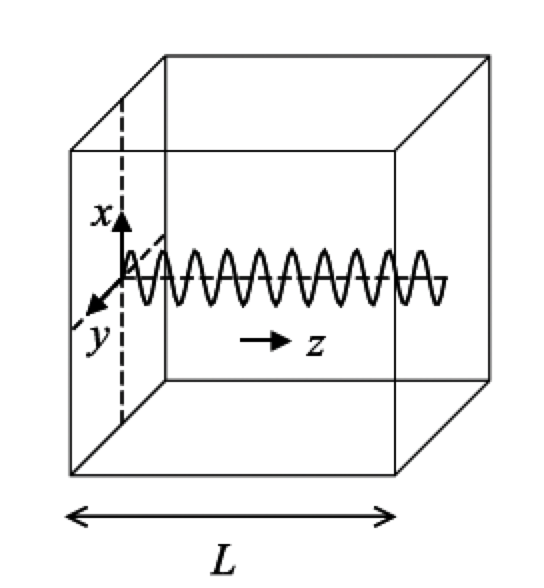
\includegraphics[width=0.22\textwidth]{figs/2022-04-27-12-37-33.png}
    \end{center}
   场分量如下:  
   \[ \begin{cases}
    E_{x}(z, t)=E_{0} \sin k z \sin \omega t \\ 
    B_{y}(z, t)=B_{0} \cos k z \cos \omega t  \quad \text{with} \quad B_{0} = E_{0} /c 
   \end{cases} \]
 \end{frame}
 
%\begin{frame}
% \frametitle{}
% 电磁场的能量密度为:
% \[ H=\frac{1}{2}\left(\epsilon_{0} {E}^{2}+\frac{1}{\mu_{0}} B^{2}\right) \]
% 电场能 (设模面积为A): 
% \[ \begin{aligned}
%  E_{\text {electric }} &=\frac{1}{2} \epsilon_{0} A \int_{0}^{L} {E}_{0}^{2} \sin ^{2} k z \sin ^{2} \omega t \mathrm{~d} z \\
%  &=\frac{1}{4} \epsilon_{0} A {E}_{0}^{2} \sin ^{2} \omega t \int_{0}^{L}(1-\cos 2 k z) \mathrm{d} z \\
%  &=\frac{1}{4} \epsilon_{0} V {E}_{0}^{2} \sin ^{2} \omega t
%  \end{aligned}
%    \]       
%\end{frame}
%
%\begin{frame}
% \frametitle{}
% 磁场能 :  
% \[\begin{aligned}
%  E_{\text {magnetic }} &=\frac{1}{2 \mu_{0}} A \int_{0}^{L} B_{0}^{2} \cos ^{2} k z \cos ^{2} \omega t \mathrm{~d} z \\
%  &=\frac{1}{4 \mu_{0}} A B_{0}^{2} \cos ^{2} \omega t \int_{0}^{L}(1+\cos 2 k z) \mathrm{d} z \\
%  &=\frac{1}{4 \mu_{0}} V B_{0}^{2} \cos ^{2} \omega t
%  \end{aligned} \] 
%总能量 :
%\[ H=\frac{V}{4}\left(\epsilon_{0} \mathcal{E}_{0}^{2} \sin ^{2} \omega t+\frac{B_{0}^{2}}{\mu_{0}} \cos ^{2} \omega t\right)
%   \]
%\end{frame}
%
%begin{frame}
% \frametitle{}
% 令: \[ q(t)=\left(\frac{\epsilon_{0} V}{2 \omega^{2}}\right)^{1 / 2} \mathcal{E}_{0} \sin \omega t \]
% \[ p(t)=\left(\frac{V}{2 \mu_{0}}\right)^{1 / 2} B_{0} \cos \omega t \equiv\left(\frac{\epsilon_{0} V}{2}\right)^{1 / 2} \mathcal{E}_{0} \cos \omega t \]
% 代回, 得总能:
%     \[ H=\frac{1}{2}\left(p^{2}+\omega^{2} q^{2}\right) \]
% 说明电磁场的振荡是电场能与磁场能之间的转换
%end{frame}

\begin{frame}
 \frametitle{}
 初始条件决定一个初始相位 $ \varphi$ \\ 
  {\Bullet}复函表示:  \[
    \begin{aligned}
         E_{x}(z, t) &=E_{0} (z) e^ {i\varphi}  \\
         &=  E_{0}(z) \cos\varphi  + i E_{0}(z) \sin\varphi \\ 
         &= E_1 (z,t) + i E_2 (z,t)
    \end{aligned}
    \]
  其中 $E_1(z,t), E_2(z,t) $是电场的实部和虚部 \\   
\end{frame}

\begin{frame}
   \begin{center}
      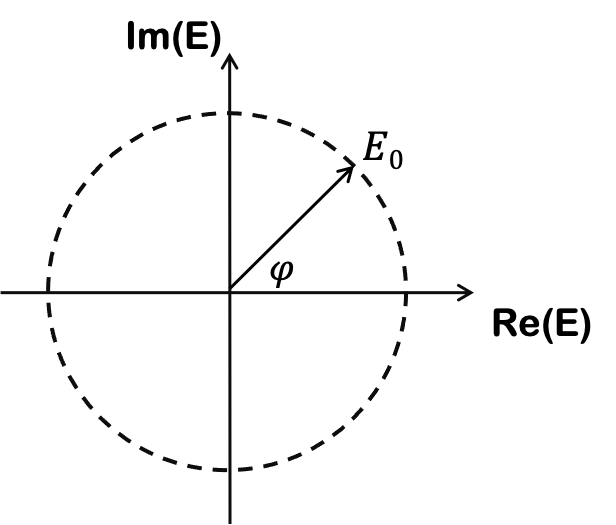
\includegraphics[width=0.4\textwidth]{figs/2.png}
   \end{center}
 \[ \begin{cases}
  Re(E)= E_{0}(z) \cos\varphi\\ 
  Im(E)= E_{0}(z) \sin\varphi\\ 
 \end{cases} \]
 电磁场的大小和相位角都是确定的.  
\end{frame}

\begin{frame}
  \frametitle{经典相图2}
  定义电场的正交分量(field quadratures)
  \[ \begin{cases}
    X_{1}(t) = \sqrt{\frac{\omega}{2\hbar}}q(t)= \sqrt{\frac{\epsilon_{0} V}{4 \hbar \omega}} {E}_{0} \sin \omega t\\ 
    X_{2}(t) = \sqrt{\frac{1}{2\hbar \omega}}p(t)= \sqrt{\frac{\epsilon_{0} V}{4 \hbar \omega}} {E}_{0} \cos \omega t\\ 
   \end{cases} \]
   代入
   \[
  \begin{aligned}
       E_{x}(z, t) &=E_{0} \sin k z \sin (\omega t + \varphi) \\
       &=  E_{0} \sin k z (\cos\varphi \sin\omega t + \sin\varphi \cos\omega t) \\ 
       &= \sqrt{\frac{4 \hbar \omega}{\epsilon_{0} V}} \sin k z\left(\cos \varphi X_{1}(t)+\sin \varphi X_{2}(t)\right) \\ 
       &=  X_{1}(z,t)+ i X_{2}(z,t)
  \end{aligned}
  \]
\end{frame}

\begin{frame}
  \begin{center}
     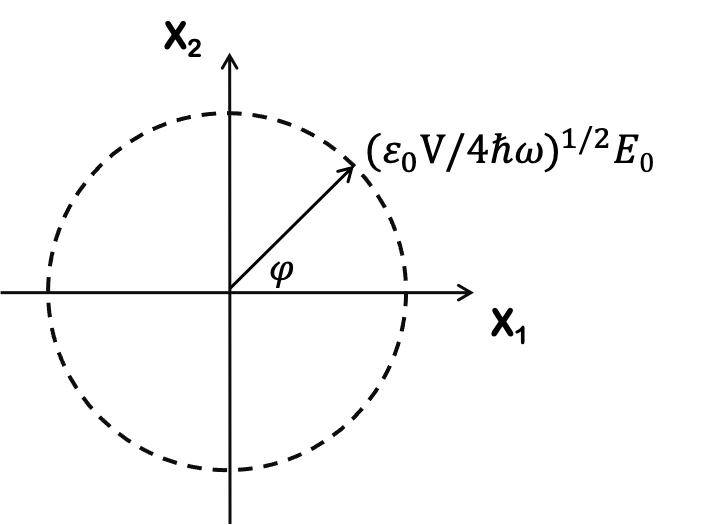
\includegraphics[width=0.5\textwidth]{figs/3.png}
  \end{center}
\end{frame}


\begin{frame}
  \frametitle{量子化相图}
  场正交分量可量子化:
  \[ \begin{cases}
    \hat{X}_{1}(t) = \sqrt{\frac{\omega_l}{2\hbar}}\hat{q}(t)=\frac{1}{2}\left(a+a^{^{\dagger}}\right)\\ 
    \hat{X}_{2}(t) = \sqrt{\frac{1}{2\hbar \omega_l}}\hat{p}(t)= \frac{1}{2 i}\left(a-a^{^{\dagger}}\right)\\ 
   \end{cases} \]
  \[ \text{with} \, [X_1, X_2] =\frac{i}{2} \]
  计算不确定度:
  \[ \Delta X_1 \Delta X_2  = \frac{1}{2\hbar}  \Delta q \Delta p \geq \frac{1}{2\hbar} \frac{\hbar}{2}=\frac{1}{4}  \]
\end{frame}

\begin{frame}
    \frametitle{} 
    \begin{center}
       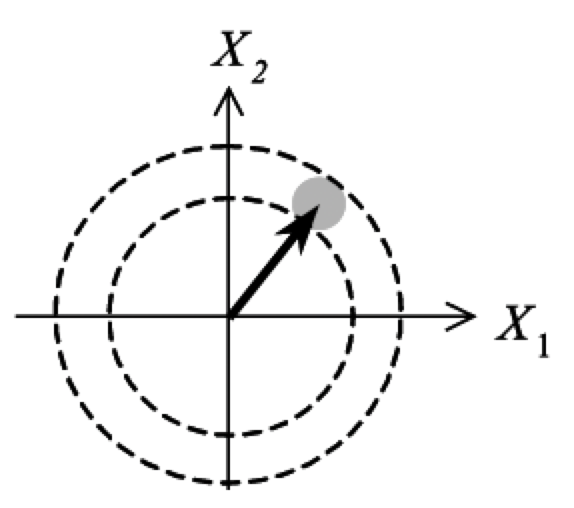
\includegraphics[width=0.4\textwidth]{figs/2022-04-27-15-34-34.png}
    \end{center}
    \[ \Delta X_1 \Delta X_2  \geq  \frac{1}{4}  \]
    电磁场的大小和相位角都有一定的不确定性. 灰色区描述不可区分的简并态. 
\end{frame}

\begin{frame}
  \frametitle{}
  \例[4.试证明真空态是最小不确定度乘积态]{
   \[ \Delta X_1 \Delta X_2 =\dfrac{1}{4}, \, \Delta X_1 = \Delta X_2 = \frac{1}{2} \] 
  }
  \解~不确定度计算公式\[ \Delta x  = \sqrt{ \overline{x^2}- \overline{x}^2}\] 
\[ 
\begin{aligned}
  \overline{ X_1}  &= \lcr{n}{\frac{1}{2}\left(a+a^{\dagger}\right)}{n} \\ 
        &= 0 \\
  \overline{ X_2 } &= \lcr{n}{\frac{1}{2i}\left(a-a^{\dagger}\right)}{n} \\ 
        &= 0 
\end{aligned}\]
\end{frame}

\begin{frame}
  \frametitle{}
\[ 
\begin{aligned}
  \overline{X_1 ^2} &= \lcr{n}{\frac{1}{4}\left(a+a^{\dagger}\right)^2}{n} \\
        &= \frac{1}{4} \lcr{n}{\left(aa+a^{\dagger}a^{\dagger}+aa^{\dagger}+ a^{\dagger}a\right)^2}{n} \\
        &= \frac{1}{4} (2n+1)
\end{aligned}\]
\[
\begin{aligned}
  \overline{X_2 ^2} &= \lcr{n}{-\frac{1}{4}\left(a-a^{\dagger}\right)^2}{n} \\
  &= -\frac{1}{4} \lcr{n}{\left(aa+a^{\dagger}a^{\dagger}-aa^{\dagger}- a^{\dagger}a\right)^2}{n} \\
  &= \frac{1}{4} (2n+1)
\end{aligned}\]
\[ \Delta X_1 = \Delta X_2  =  \sqrt{ \overline{X^2}- \overline{X}^2} =\frac{1}{2}\sqrt{2n+1}\geq \frac{1}{2}\] 
\end{frame}

\begin{frame}
 \frametitle{}
  对于真空态
 \[ \Delta X_1 = \Delta X_2  = \frac{1}{2}\]
 \[ \Delta X_1 \Delta X_2  = \frac{1}{4}\]    
 证毕!\\ 
\end{frame}

\begin{frame}
 \frametitle{真空态相图}
真空态的经典电场能$E_0=0$, 电场矢量大小为零, 处于原点.  
      \begin{center}
         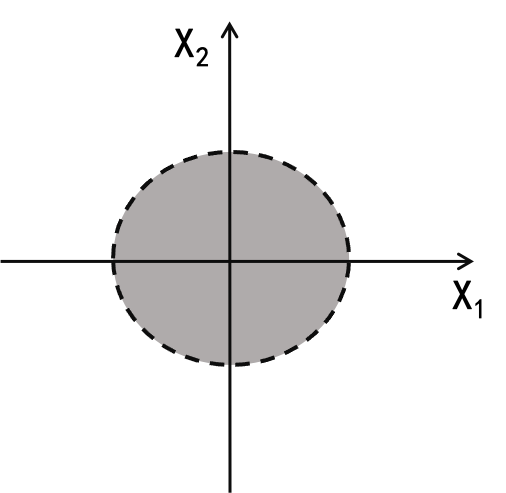
\includegraphics[width=0.4\textwidth]{figs/4.png}
      \end{center}
      \[ \Delta X_1 = \Delta X_2  = \frac{1}{2}\]
真空态的量子涨落为量子噪音的极限(极小值$\dfrac{1}{4}$), 是场强完全确定而相位完全不确定的态. 
\end{frame}

\begin{frame} 
\frametitle{小结:}
  (1) 光场哈密顿可表示为一系列量子化的场谐振子的能量 (一次量子化)
  \[ \hat{H}_{k\sigma}= \sum_{k,\sigma}\hbar \omega_{k\sigma} \left(\hat{a}^\dagger _{k\sigma} \hat{a} _{k\sigma}+ \frac{1 }{2}\right) \qquad \text{with} \quad [\hat{a} _{k\sigma},\hat{a}^\dagger _{k\sigma}]=1 \]
  (2) 自由光场的电场可表示为一系列量子化的平面波 (二次量子化)
  \[\begin{aligned}
    \hat{\mathbf{E}} (\mathbf{r},t) &=i \sum^\infty _{k,\sigma} (\frac{\hbar\omega_k}{2 \epsilon_0 V } )^{1/2} \hat{e}_\sigma \left[ \hat{a} _{k\sigma} (t) e^{i \mathbf{k}\cdot \mathbf{r}} - \hat{a} ^\dagger _{k\sigma} (t)  e^{-i \mathbf{k}\cdot \mathbf{r}}\right] \\
    &= \hat{\mathbf{E}}^+(\mathbf{r},t)+ \hat{\mathbf{E}}^-(\mathbf{r},t)
  \end{aligned} \]
\end{frame}
%%%%%%%%%%%%%%%%%%%%%%%%%%%%%%%%%%%%%%%%%%%%%%%%%%%%%%%%%%%%%%%%%%%
\begin{frame}
    \frametitle{课外作业}
    \begin{enumerate}
        \item  利用腔模正交性证明 \[ H= \sum_l H_l\]
        \item  计算电磁场真空态的量子涨落
    \end{enumerate}
\end{frame}
%%%%%%%%%%%%%%%%%%%%%%%%%%%%%%%%%%%%%%%%%%%%%%%%%%%%%%%%%%%%%%%%%%%